\subsection[Splitting data]{Splitting data}

\subsubsection[Training e test set]{Training e test set}


\begin{frame}

	\frametitle{Split dei dati: training e test set}

	Ma un modello di machine learning mira a fare \textbf{buone previsioni su dati nuovi} e mai visti prima.
	Ma se stai costruendo un modello dal tuo dataset, come potresti ottenere dei dati precedentemente non visti?\vspace{3mm}
	\pause

	Un modo è \textbf{dividere il dataset in due sottoinsiemi}:
	\begin{itemize}
		\item \textbf{training-set}, un sottoinsieme per addestrare un modello
		\item \textbf{test-set}, un sottoinsieme per testare il modello addestrato
	\end{itemize}
	\ \\
	Una buona prestazione sul test set è un utile indicatore di buone prestazioni su dei nuovi dati in generale, supponendo che:
	\begin{itemize}
		\item il test-set sia abbastanza grande per produrre risultati statisticamente significativi
		\item non imbrogli usando lo stesso test-set più e più volte
		\item è rappresentativo dell'insieme di dati nel suo complesso
	\end{itemize}
\end{frame}


\begin{frame}

	\frametitle{Split dei dati: training e test set}

	Supponendo che il set di test soddisfi le condizioni precedenti, l'obiettivo è creare un modello che generalizzi bene sui nuovi dati.\\
	Il nostro test set funge da proxy per i nuovi dati.
	\newlinedouble
	Ad esempio, consideriamo la seguente immagine:
	\begin{figure}[!htbp]
		\centering
		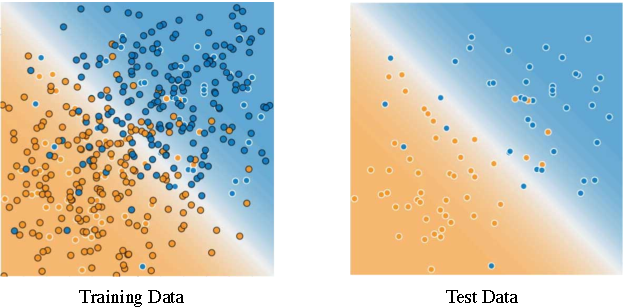
\includegraphics[width=0.8\linewidth]{images/supervised/validation_test_splitting_data/TrainingDataVsTestData.pdf}
%				\caption{Alberi malati (in blu) e sani (in rosso)}
%				\label{}
	\end{figure}

%	\begin{columns}
%			\column{0.55\linewidth}
%%			Un semplice caso di overfitting: le linee verdi e nere rappresentano modelli di classificazione overfitting e non-overfitting. La linea verde classifica perfettamente i dati del training-set, ma sembra che sia troppo dipendente da quei dati (memorizzazione dei dati / memorizing the data).\\
%%			È molto probabile che la linea verde abbia un tasso di errore più elevato sui nuovi dati non visualizzati, rispetto alla linea nera.
%
%			Per sviluppare un po' di intuizione su questo concetto, guarderemo tre figure.
%			\newlinedouble
%			Supponiamo che ogni punto in queste figure rappresenti la posizione di un albero in una foresta.\\
%			I due colori hanno i seguenti significati:
%			\begin{itemize}
%				\item I punti blu rappresentano alberi malati
%				\item I punti rossi rappresentano alberi sani
%			\end{itemize}
%
%			\column{0.45\linewidth}
%			\begin{figure}[!htbp]
%				\centering
%				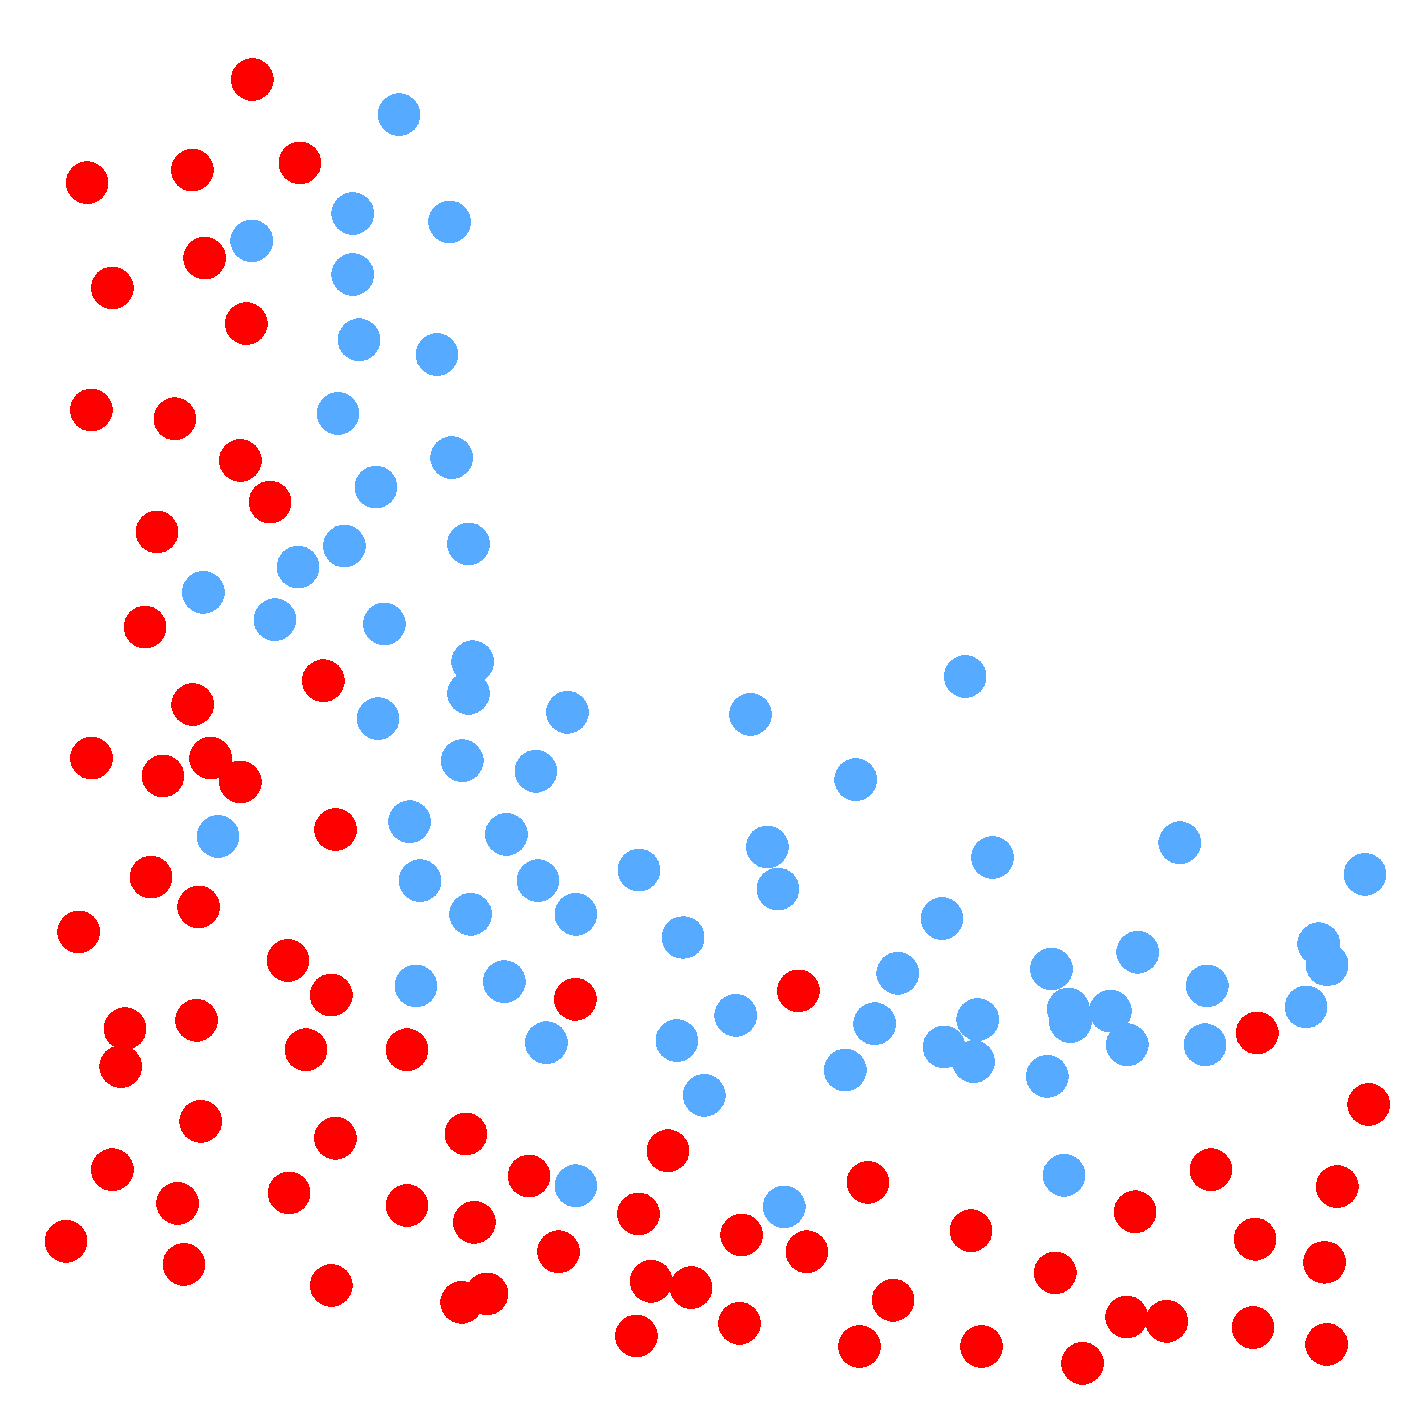
\includegraphics[width=1.0\linewidth]{images/supervised/validation_test_training_peril_of_overfitting/overfitting.png}
%%				\caption{Alberi malati (in blu) e sani (in rosso)}
%%				\label{}
%			\end{figure}
%
%	\end{columns}
\end{frame}


\begin{frame}

	\frametitle{Split dei dati: training e test set}

	\begin{figure}[!htbp]
		\centering
		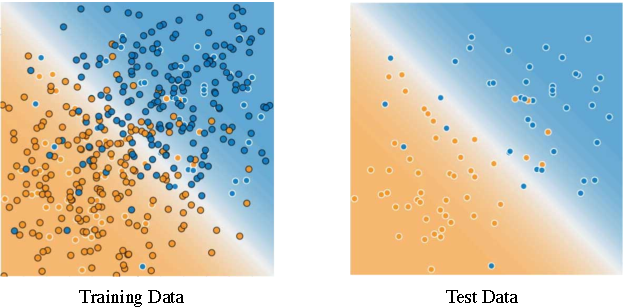
\includegraphics[width=0.8\linewidth]{images/supervised/validation_test_splitting_data/TrainingDataVsTestData.pdf}
%				\caption{Alberi malati (in blu) e sani (in rosso)}
%				\label{}
	\end{figure}
	Si noti che il modello appreso attraverso il training set è molto semplice.\\
	Questo modello \textbf{non fa un lavoro perfetto}: alcune previsioni sono sbagliate.
	\textbf{Tuttavia}, questo modello funziona tanto sui dati di test quanto sui dati di addestramento. In altre parole, questo semplice modello \textbf{non si adatta ai dati di addestramento}.
\end{frame}


\begin{frame}

	\frametitle{Mai addestrare sul test set}

	\begin{columns}
			\column{0.7\linewidth}
			Se ottieni risultati sorprendentemente buoni nelle tue metriche di valutazione, potrebbe darsi che stai \textbf{accidentalmente allenando il modello sul test set}.
			\newlinedouble
			Ad esempio, un'elevata precisione potrebbe indicare che i dati di test sono trapelati nel set di addestramento.
			\newlinedouble
			Ad esempio, si consideri un modello che prevede se un'e-mail è spam, utilizzando la riga dell'oggetto, il corpo dell'e-mail e l'indirizzo e-mail del mittente come features.

			\column{0.3\linewidth}
			\begin{figure}[!htbp]
				\centering
				
\includegraphics[width=1.0\linewidth]{images/supervised/validation_test_splitting_data/spam_filter.jpg}
%				\caption{Alberi malati (in blu) e sani (in rosso)}
%				\label{}
			\end{figure}

	\end{columns}

\end{frame}


\begin{frame}

	\frametitle{Mai addestrare sul test set: esempio dello filtro spam}

	\begin{columns}
			\column{0.7\linewidth}
			\begin{itemize}
				\item suddividiamo i dati in set di addestramento e test, con una suddivisione di 80-20
				\item dopo l'addestramento, il modello raggiunge una precisione del 99\% su train e test set
				\item ci aspetteremmo una precisione inferiore sul test-set, quindi diamo un'altra occhiata ai dati e scopriamo che molti degli esempi nel set di test sono duplicati di esempi nel set di addestramento%(abbiamo trascurato di pulire le voci duplicate per lo stesso spam email dal nostro database di input prima di suddividere i dati)
				\item abbiamo inavvertitamente eseguito il training su alcuni dei nostri dati di test e, di conseguenza, non stiamo più misurando accuratamente quanto bene il nostro modello si generalizza su dei nuovi dati
			\end{itemize}

			\column{0.3\linewidth}
			\begin{figure}[!htbp]
				\centering
				
\includegraphics[width=1.0\linewidth]{images/supervised/validation_test_splitting_data/spam_filter.jpg}
%				\caption{Alberi malati (in blu) e sani (in rosso)}
%				\label{}
			\end{figure}

	\end{columns}


\end{frame}


\begin{frame}

	\frametitle{Split dei dati: training e test set}
	\begin{columns}
			\column{0.55\linewidth}
			Il partizionamento del dataset in \textbf{training} e \textbf{test set} per mette quindi di addestrare il modello su un set di esempi e quindi di testare il modello su un diverso set di esempi.
			\newlinedouble
			Con \textbf{queste due partizioni}, il flusso di lavoro potrebbe essere quello mostrato in figura.
			\newlinedouble
			Dividere il dataset in due set è una buona idea, ma non una panacea.
			% Nella figura, "Modifica modello" significa modificare qualsiasi cosa sul modello che puoi immaginare: dalla modifica del tasso di apprendimento, all'aggiunta o alla rimozione di funzionalità, alla progettazione di un modello completamente nuovo da zero. Alla fine di questo flusso di lavoro, scegli il modello che funziona meglio sul set di test.

			\column{0.45\linewidth}
			\begin{figure}[!htbp]
				\centering
				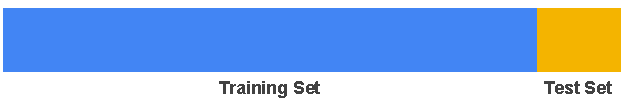
\includegraphics[width=1.0\linewidth]{images/supervised/validation_test_splitting_data/Training_Test_1.pdf}
				\caption{Split training, validation e test set}
			\end{figure}

			\begin{figure}[!htbp]
				\centering
				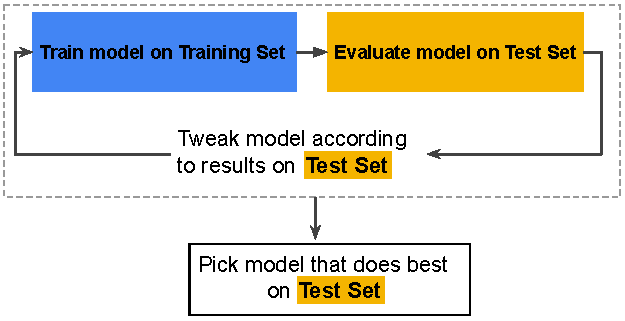
\includegraphics[width=1.0\linewidth]{images/supervised/validation_test_splitting_data/Training_Test_2.pdf}
				\caption{Workflow training, validation e test set}
			\end{figure}

	\end{columns}
\end{frame}



\subsubsection[Validation set]{Validation set}


\begin{frame}

	\frametitle{Split dei dati: training, validation e test set}
	\begin{columns}
		\column{0.55\linewidth}
		È possibile ridurre le possibilità di overfitting partizionando il set di dati nei \textbf{tre sottoinsiemi} mostrati nella figura mostrata in alto a destra.
		\newlinedouble

		La figura in basso a destra mostra il nuovo flusso di lavoro utilizzando questi tre sottoinsiemi:
		\begin{itemize}
			\item usare il validation set per valutare i risultati dell'addestramento sul training-set
			\item se il modello ha ``superato'' il test sul validation set
			\item allora utilizzare il test set per ricontrollare la valutazione
		\end{itemize}


		\column{0.45\linewidth}
		\begin{figure}[!htbp]
			\centering
			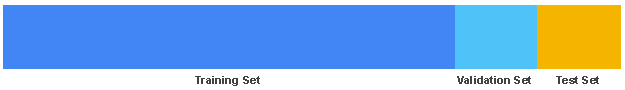
\includegraphics[width=1.0\linewidth]{images/supervised/validation_test_splitting_data/Training_Test_Validation_1.pdf}
			\caption{Split training e test set}
		\end{figure}

		\begin{figure}[!htbp]
			\centering
			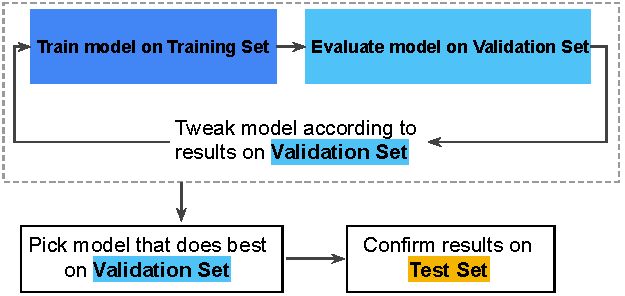
\includegraphics[width=1.0\linewidth]{images/supervised/validation_test_splitting_data/Training_Test_Validation_2.pdf}
			\caption{Workflow training e test set}
		\end{figure}
	\end{columns}
\end{frame}


\begin{frame}

	\frametitle{Split dei dati: training, validation e test set}
	\begin{columns}
		\column{0.55\linewidth}
		In questo flusso di lavoro quindi si procede nel seguente modo:
		\begin{itemize}
			\item si sceglie il modello che funziona meglio sul validation set
			\item si ricontrolla il comportamento di quel modello sul test set
		\end{itemize}
		% Questo è un flusso di lavoro migliore perché crea meno esposizioni al set di test.


		\column{0.45\linewidth}
		\begin{figure}[!htbp]
			\centering
			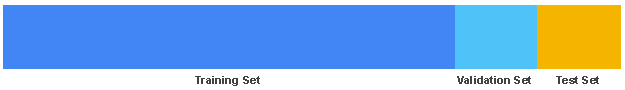
\includegraphics[width=1.0\linewidth]{images/supervised/validation_test_splitting_data/Training_Test_Validation_1.pdf}
			\caption{Split training e test set}
		\end{figure}

		\begin{figure}[!htbp]
			\centering
			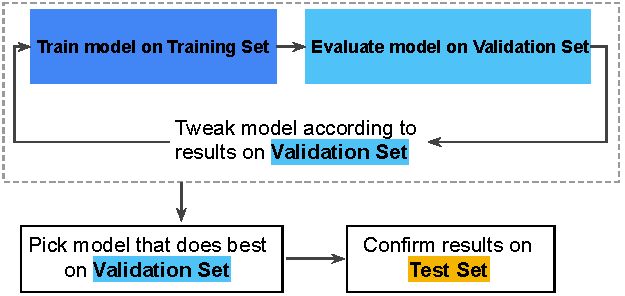
\includegraphics[width=1.0\linewidth]{images/supervised/validation_test_splitting_data/Training_Test_Validation_2.pdf}
			\caption{Workflow training e test set}
		\end{figure}

	\end{columns}
\end{frame}


\begin{frame}

	\frametitle{Workflow con training, validation e test set}
	\begin{figure}[!htbp]
		\centering
		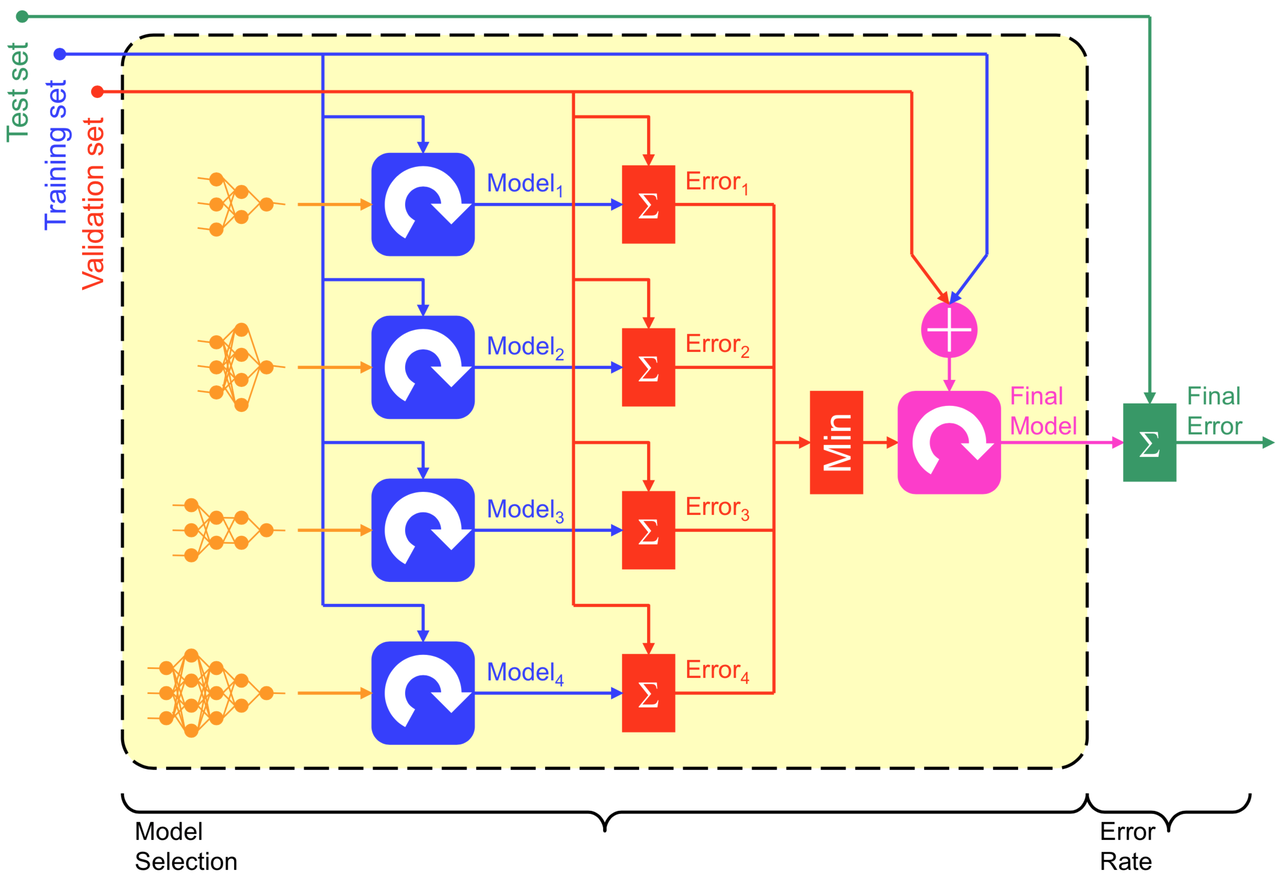
\includegraphics[width=0.85\linewidth]{images/supervised/validation_test_splitting_data/Workflow.png}
%		\caption{Split training e test set}
	\end{figure}
\end{frame}




\subsubsection[K-fold Cross-Validation]{K-fold Cross-Validation (K-CV)}

\begin{frame}

	\frametitle{K-fold Cross-Validation}

	L'ultimo approccio visto non è sempre praticabile, o desiderabile.\\
	Di solito richiede di disporre di un dataset piuttosto grande.
	\newlinedouble
	I metodi di \emph{ricampionamento} sono strumenti che:
	\begin{itemize}
		\item permettono di ricampionare \emph{ripetutamente} dallo stesso training set, e
		\item ristimare il modello di interesse su ciascun campione artificiale
		\item per ottenere maggiore informazione sul modello stimato o per migliorare il suo adattamento ai dati
	\end{itemize}
	\ \\
	Per molto tempo la \textbf{cross-validation} e il \textbf{bootstrap} sono stati considerati dei metodi computazionalmente troppo onerosi -- ora non più, grazie alla potenza di calcolo dei moderni PC.
	\newline
	L'idea della cross-validation è quella di \emph{escludere iterativamente} un sottoinsieme delle osservazioni ed usarlo come campione di test.
\end{frame}


\begin{frame}
	\frametitle{$K$-fold Cross-Validation}
	\begin{itemize}
		\item La $K$-CV è una delle tecniche più utilizzate per stimare l'errore di test
		\item Idea:
		\begin{itemize}
			\item[--] suddividere casualmente il campione in $K$ sottoinsiemi disgiunti e di uguale numerosità
			\item[--] per $k=1,2,\ldots,K$:
				\begin{itemize}
					\item escludiamo uno dei sottocampioni e addestriamo il modello sui rimanenti $K-1$
					\item usando il modello stimato prevediamo la variabile risposta sul sottocampione non usato per la stima
				\end{itemize}
			\item[--] stimiamo l'errore di test usando la media degli errori calcolati nei $K$ passi precedenti
		\end{itemize}

		\item È meglio mantenere fissi i $K$ sottocampioni, piuttosto che ricampionarli casualmente in ognuno dei $K$ passi:
		\begin{enumerate}
			\item in questo modo non saremmo sicuri che ciascuna osservazione sia esclusa dalla stima solo una volta
			\item la casualità addizionale amplifica la varianza dei risultati della CV
		\end{enumerate}
	\end{itemize}
\end{frame}


\begin{frame}
	\frametitle{$K$-CV per problemi di regressione}
	\begin{itemize}
		\item Sia $C_k$ l'insieme degli indici delle $n_k$ osservazioni nel sottocampione $k=1,2,\ldots,K$

		\item Per $k=1,2,\ldots,K$, calcoliamo
		\[
		\mbox{MSE}_k = \frac{1}{n_k}\sum_{i\in C_k} (y_i-\hat y_i)^2
		\]
		dove $\hat y_i$ è la previsione dell'osservazione $i$ usando il modello stimato sul campione che esclude il sottocampione $k$

		\item Per calcolare una stima dell'errore di test del modello, calcoliamo la media degli errori quadratici relativi ai $K$ sottocampioni:
		\[
		\mbox{CV}_{(K)} = \sum_{k=1}^K \frac{n_k}{n}\,\mbox{MSE}_k
		\]
	\end{itemize}
\end{frame}


\begin{frame}
	\frametitle{Cross-Validation per problemi di classificazione}

	\begin{itemize}
		\item In un problema di classificazione possiamo misurare l'errore di test nel sottocampione $k$-esimo usando l'errore di classificazione totale:
		\[
		\mbox{Err}_{(k)} = \frac{1}{n_k}\sum_{i\in C_k} \mathbb{I}(y_i\not= \hat y _i)
		\]

		\item Iteriamo sui $K$ sottocampioni e calcoliamo la media:
		\[
		\mbox{CV}_{(K)} = \sum_{k=1}^K \frac{n_k}{n} \, \mbox{Err}_{(k)}
		\]

		\item Più in generale, oltre a stimare l'\emph{errore di test atteso}, possiamo anche stimare lo \emph{scarto quadratico medio} di $\mbox{CV}_{(K)}$:
		\[
		\widehat{\se}[\mbox{CV}_{(K)}] = \sqrt{\frac{1}{K} \sum_{k=1}^K \frac{(\mbox{Err}_{(k)}-\overline{\mbox{Err}})^2}{K-1}}
		\]

		%\item Notare tuttavia che $\widehat{\se}[\mbox{CV}_{(K)}]$ non tiene conto della correlazione fra $\mbox{Err}_{(k)}$, $k=1,2,\ldots,K$
	\end{itemize}
\end{frame}


\begin{frame}

	\frametitle{$K$-fold Cross-Validation}
	\begin{figure}[!htbp]
		\centering
		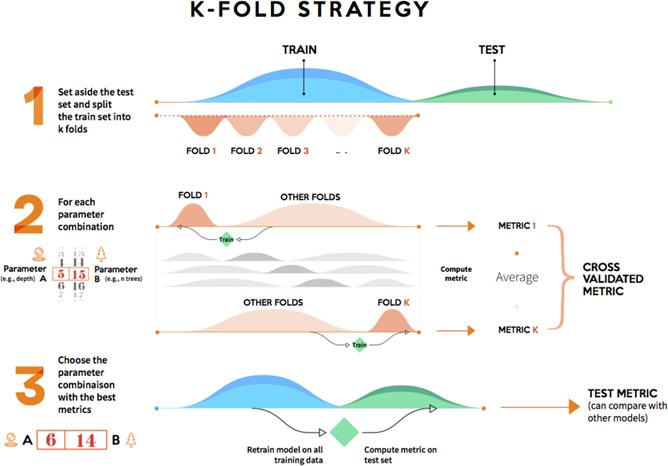
\includegraphics[width=0.85\linewidth]{images/supervised/validation_test_splitting_data/Kfold.jpg}
%		\caption{Split training e test set}
	\end{figure}
\end{frame}


\begin{frame}
	\frametitle{$K$-CV: Problemi}
	\begin{itemize}
		\item Può essere \emph{lenta}: il modello deve essere addestrato $K$ volte
		\item Può fornire stime \emph{distorte}, dato che ciascuno dei $K$ campioni di addestramento contiene solo una frazione $(K - 1)/K$ delle osservazioni nel dataset originale (\emph{minore sovrastima rispetto a validation set})
		%\item Suddivisioni diverse continuano a fornire risultati potenzialmente contrastanti -- ma molto meno che nell'approccio del validation set (\emph{minore varianza rispetto a validation set})
		\item $K$-CV può tuttavia essere \emph{instabile} i risultati possono cambiare in maniera significativa da un campione all'altro% (dipende dalla stabilità del metodo di stima)
		% -- in altre parole, può avere varianza campionaria molto elevata --
		% \item È necessario fare attenzione ad alcuni errori involontari -- v. oltre
		\item In pratica, $K = 5$ o 10 sono i valori di $K$ tipici
	\end{itemize}
\end{frame}





\subsubsection[Leave-One-Out Cross-Validation]{Leave-One-Out Cross-Validation  (LOOCV)}
\begin{frame}
	\frametitle{Leave-One-Out CV (LOOCV)}
	\begin{itemize}
		\item Ponendo $K=n$ otteniamo la \emph{Leave-One-Out Cross-Validation}
		\item LOOCV può essere estremamente onerosa in termini di complessità computazionale, ma nel caso dei minimi quadrati equivale a un'unica stima del modello:
		\[
		\mbox{CV}_{(n)} = \frac{1}{n} \sum_{i=1}^n \left(\frac{y_i-\hat y_i}{1-h_i}\right)^2
		\]
		dove
		\begin{itemize}
			\item $\hat y_i$ è la $i$-esima previsione dei minimi quadrati \emph{originari}

			\item $h_i$ è il ``leverage'' -- l'elemento $(i,i)$ di $\mbP=\mbX(\mbX^\prime \mbX)^{-1} \mbX$
		\end{itemize}

		\item Notare che, dato il campione, la LOOCV è deterministica
		%\item Ovviamente LOOCV minimizza la distorsione della CV
		%\item In compenso, gli $n$ campioni d'addestramento sono quasi identici, il che significa che gli $n$ errori quadratici medi sui campioni di test sono molto correlati fra loro. Di conseguenza, la loro media può avere varianza elevata
	\end{itemize}
\end{frame}


\begin{frame}

	\frametitle{Leave-One-Out CV (LOOCV)}
	\begin{figure}[!htbp]
		\centering
		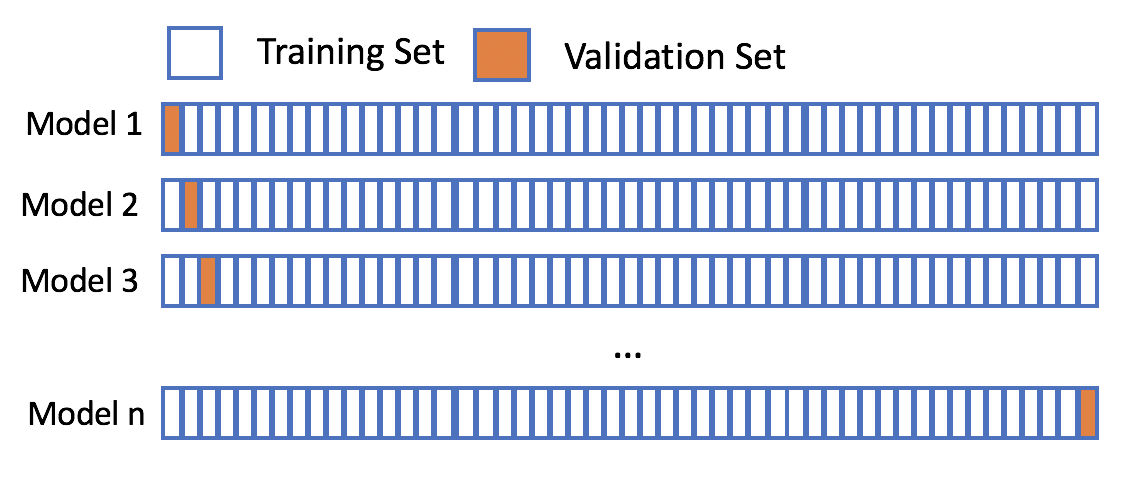
\includegraphics[width=0.90\linewidth]{images/supervised/validation_test_splitting_data/loocv.png}
%		\caption{Split training e test set}
	\end{figure}
\end{frame}



%\begin{frame}
%	\frametitle{Come \emph{non} effettuare la CV}
%	\begin{itemize}
%		\item Consideriamo un problema di classificazione binaria, con $n=1000$ e $p=500$
%
%		\item Per ridurre il numero di predittori potremmo decidere di adottare la strategia seguente:
%		\begin{enumerate}
%			\item Individuiamo i 100 predittori con correlazione massima con $Y$
%
%			\item Applichiamo un classificatore (per esempio la regressione logistica) usando solo questi 100 predittori
%		\end{enumerate}
%
%		\item Possiamo stimare l'errore di test di questo classificatore applicando la CV al solo passo 2, dimenticandoci del passo 1?
%
%		\item NO: In questo modo ignoreremmo il fatto che il passo 1 \emph{è una forma di apprendimento}: la procedura \emph{usa la $Y$ nel campione di addestramento}
%
%		\item Per questo motivo il passo 1 \emph{deve} essere incluso nella procadura di CV
%
%		\item Potremmo modificare il passo 1. precedente nel modo seguente:
%		\begin{enumerate}
%			\item Individuiamo i 100 predittori con varianza campionaria massima
%		\end{enumerate}
%		In questo caso il passo 1. non deve necessariamente essere incluso nella procedura di CV
%	\end{itemize}
%\end{frame}


\subsubsection[Bootstrap]{Bootstrap}

\begin{frame}

	\frametitle{Bootstrap}
	Un'altra delle metodologie utilizzate per ridurre l'overfitting nella scelta del modello è il	 \textbf{bootstrap}.
	\newlinedouble
	Dato un training set $D$ di dimensione $n$, il bagging genera $m$ nuovi training sets $D_i$, ognuno di dimensione $n'$, campionando da $D$ uniformemente e con reinserimento.\\
	Campionando con reinserimento, alcune osservazioni possono essere ripetute in ogni $D_i$.
	\begin{itemize}
		\item[--] il bootstrap, imita la generazione di nuovi campioni
		\item[--] i \emph{campioni bootstrap} sono ottenuti campionando ripetutamente le osservazioni nel dataset disponibile \emph{con reinserimento}
		\item[--] ogni campione bootstrap contiene \emph{lo stesso numero di osservazioni}
	\end{itemize}

\end{frame}


\begin{frame}

	\frametitle{Bootstrap}
	\begin{figure}[!htbp]
		\centering
		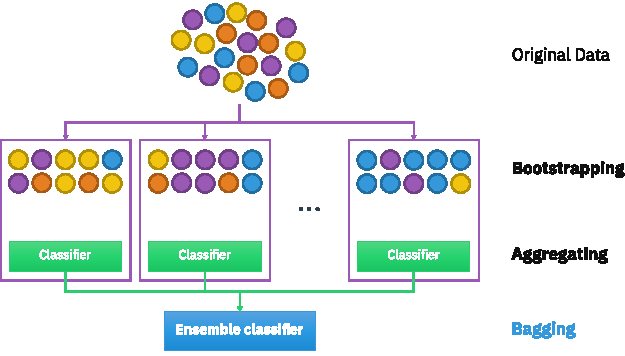
\includegraphics[width=0.9\linewidth]{images/supervised/validation_test_splitting_data/Ensemble_Bagging.pdf}
%		\caption{Split training e test set}
	\end{figure}

\end{frame}

\begin{frame}

	\frametitle{Splitting Data: i vari metodi a confronto}
	\begin{figure}[!htbp]
		\centering
		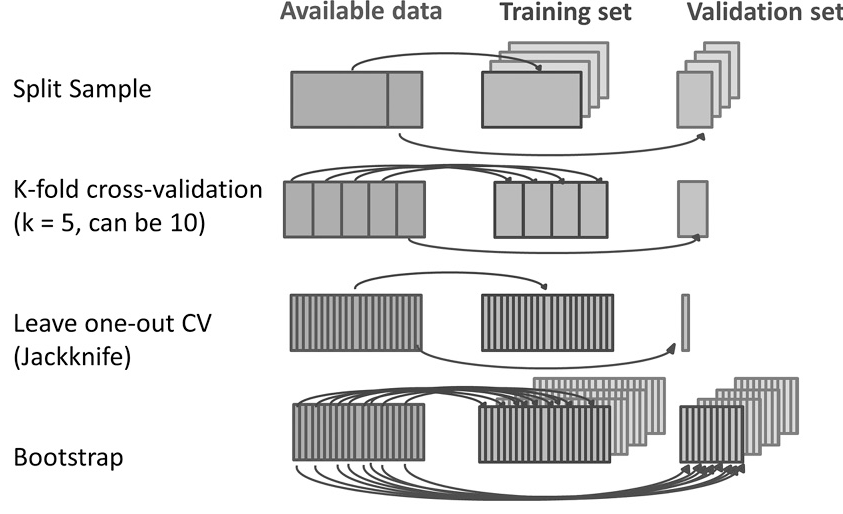
\includegraphics[width=0.9\linewidth]{images/supervised/validation_test_splitting_data/resampling_methods.png}
%		\caption{Split training e test set}
	\end{figure}

\end{frame}
